\documentclass{beamer}
%Information to be included in the title page:
\title{Exploring Shor's Algorithm}
\author{David Radcliffe}
\institute{MinneQuantum}
\date{\today}
\usetheme{AnnArbor}
\usepackage{graphicx}
\usepackage{svg}
\usepackage[utf8]{inputenc}
\usepackage{amsmath}

\begin{document}

\newcommand{\ket}[1]{\left| #1 \right\rangle}

\frame{\titlepage}

% \begin{frame}{Table of Contents}
%     \tableofcontents
% \end{frame}

\begin{frame}
    \frametitle{Outline}
    \begin{itemize}
        \item Review of quantum information theory
        \item Timeline of integer factorization
        \item Shor's algorithm
        \item Quantum order finding
        \begin{itemize}
            \item Quantum Fourier transform
            \item Quantum phase estimation
            \item Continued fractions
        \end{itemize}
    \end{itemize}
\end{frame}

\section{Quantum Information Theory}

\begin{frame}
\frametitle{Qubits}

\begin{enumerate}
    \item A qubit (quantum bit) is the basic unit of quantum 
    information
    \item While a classical bit can only be $\ket0$ or $\ket1$, 
    a qubit can exist in a superposition of $\ket0$ and $\ket1$
    \item When a qubit is measured, the outcome is either 
    $\ket0$ or $\ket1$
\end{enumerate}
\begin{figure}
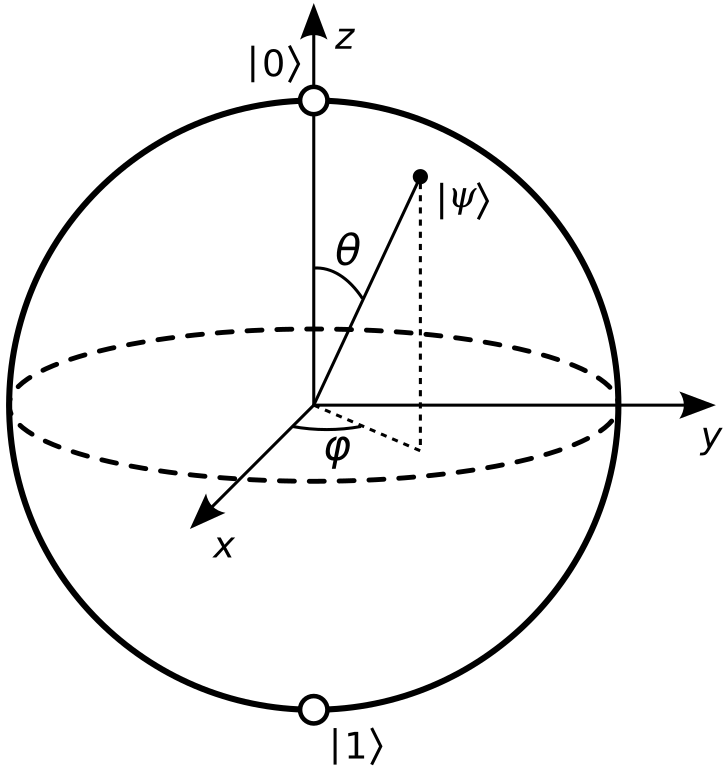
\includegraphics[height=4cm]{Bloch_sphere.svg.png}
\end{figure}
\end{frame}



\begin{frame}
\frametitle{Qubit measurement}
\begin{enumerate}
    \item If we have a qubit in the state $\ket{\psi} = \alpha \ket0 + \beta \ket1$, where $\alpha$ and $\beta$ are complex numbers, then:
    \item The probability of measuring $\ket0$ is $|\alpha|^2$
    \item The probability of measuring $\ket1$ is $|\beta|^2$
    \item $|\alpha|^2 + |\beta|^2 = 1$ because probabilities must add to 1
    \item After measurement, the qubit is in the state that was observed
\end{enumerate}

\end{frame}



\begin{frame}
\frametitle{$n$-qubit systems}
\begin{enumerate}

    \item A quantum system with $n$ qubits has $2^n$ basis states.
    \item Each basis state corresponds to a possible classical configuration of the qubits,
    represented as a binary string of length $n$.

\end{enumerate}

Examples:

\begin{enumerate}
    \item A 1-qubit system has 2 basis states: $\ket0$ and $\ket1$
    \item A 2-qubit system has 4 basis states: $\ket{00}$, $\ket{01}$, $\ket{10}$, $\ket{11}$
    \item A 3-qubit system has 8 basis states: $\ket{000}$ through $\ket{111}$
\end{enumerate}

\vskip 0.5cm

We often write these states using decimal notation: $\ket0, \ket1, \ket2, \ket3$, and so on.


\end{frame}



\begin{frame}
\frametitle{Quantum superposition}
\begin{enumerate}
    \item A quantum state is a superposition of basis states
    \item Each basis state has an associated complex number called its amplitude
    \item The sum of their squared magnitudes equals 1
\end{enumerate}

When we measure a quantum state:
\begin{enumerate}
    \item The result is always one of the basis states
    \item The probability of measuring a particular basis state $\ket{s}$ is $|\alpha|^2$, where $\alpha$ is that state's amplitude
    \item The measurement disturbs the quantum state, collapsing it to the observed basis state
\end{enumerate}

\end{frame}

\section{Number theory}

\begin{frame}
\frametitle{History of integer factorization}

\begin{itemize}
\item Euclid (c. 300 BC) - Unique factorization, GCD algorithm
\item Fermat (1643) - Fermat Factorization Method. 
$M = a^2 - b^2 = (a - b) (a + b)$
\item Euler (1763) - Euler's totient function
\item Gauss (1801) - Modular arithmetic, congruences
\item Kraitchik (1920s) - Congruence of squares method: \\
      If $M$ divides $a^2 - b^2$ but not $a\pm b$,
      then $\gcd(a-b, M)$ and $\gcd(a+b, M)$ are 
      non-trivial factors of $M$
    \end{itemize}
\end{frame}

\begin{frame}
\frametitle{Recent history of integer factorization}
\begin{itemize}

\item Miller (1976) - Reduction of factorization to order finding
\item Rivest, Shamir, Adleman (1977) - RSA encryption
\item Dixon (1981) - Quadratic sieve algorithm (up to 100 digits)
\item Shor (1994) - Quantum algorithm for integer factorization
\item Pollard (1998) - Number field sieve algorithm (over 100 digits)
\item Boudot, et al (2020) - RSA-250 factored using GNFS
\end{itemize}
\end{frame}

\begin{frame}
\frametitle{RSA encryption}

RSA encryption is used to secure communications over the internet.

\begin{enumerate}
    \item Compute $M = p \cdot q$, where $p$ and $q$ are large primes
    \item Compute the totient: $\phi(M) = (p-1)(q-1)$
    \item Choose a public exponent $e$ such that $1 < e < \phi(M)$ and $\gcd(e, \phi(M)) = 1$
    \item Compute the private exponent $d$ such that $(d \cdot e) \bmod{\phi(M)} = 1$
    \item The public key is $(M, e)$ and the private key is $d$
    \item To encrypt a message $m$, compute $c = m^e \bmod{M}$
    \item To decrypt a ciphertext $c$, compute $m = c^d \bmod{M}$
    \item The security of RSA relies on the difficulty of factoring large numbers
\end{enumerate}
\end{frame}

\begin{frame}
\frametitle{Multiplicative order}
Assume that $\gcd(a, M) = 1$. 
If we compute successive powers 
$$1, a, a^2, a^3, \ldots$$
we will eventually see a repetition.

The order of $a$ mod $M$ is the smallest positive 
integer $r$ such that $a^r \equiv 1 \pmod{M}$.

Example: Compute the order of 2 mod 15.
\begin{itemize}
    \item $2^1 \equiv 2$
    \item $2^2 \equiv 4$
    \item $2^3 \equiv 8$
    \item $2^4 \equiv 1 \pmod{15}$, so $r = 4$.
\end{itemize}

\end{frame}


\begin{frame}
\frametitle{Example: Powers of 2 mod 91}
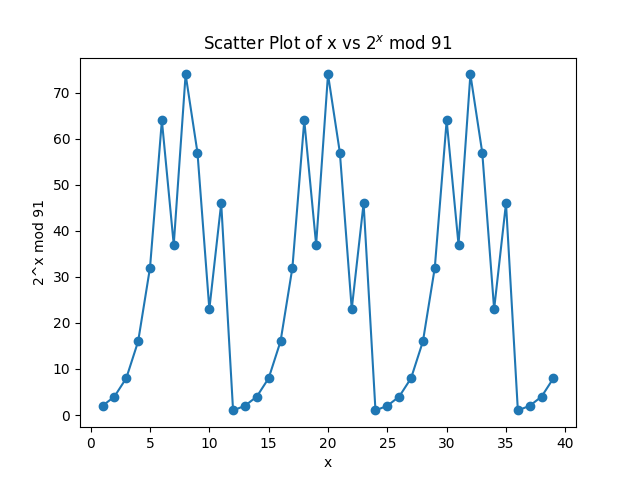
\includegraphics[height=7.5cm]{mult-order.png}


\end{frame}

\begin{frame}
\frametitle{Outline of Shor's Algorithm}
Given a composite integer $M$, Shor's algorithm finds a non-trivial factor of $M$ 
with high probability.
\begin{enumerate}
    \item Choose a random integer $a$ such that $1 < a < M$.
    \item Compute the greatest common divisor of $a$ and $M$. \\ 
    If $\gcd(a, M) > 1$, then we are done.
    \item Compute the order $r$ of $a$ mod $M$. (How???)
    \item If $r$ is even, then $M$ divides
    $a^r - 1 = \left(a^{r/2} - 1\right) \left(a^{r/2} + 1 \right)$. \\
    Compute $x = a^{r/2} \pmod{M}$.
    \item If $m$ is odd, or if $x = M - 1$, go back to step 1.
    \item Compute $\gcd(x - 1, M)$ and $\gcd(x + 1, M)$.
\end{enumerate}
\end{frame}




\section{Quantum Algorithms}

\begin{frame}
    \frametitle{Quantum Fourier Transform}

    The quantum Fourier transform (QFT) is defined by
    $$\ket{j} \mapsto \frac{1}{\sqrt{N}} \sum_{k=0}^{N-1} e^{2\pi i j k / N} \ket{k}$$
    where $N = 2^n$ is the number of basis states in the system.


    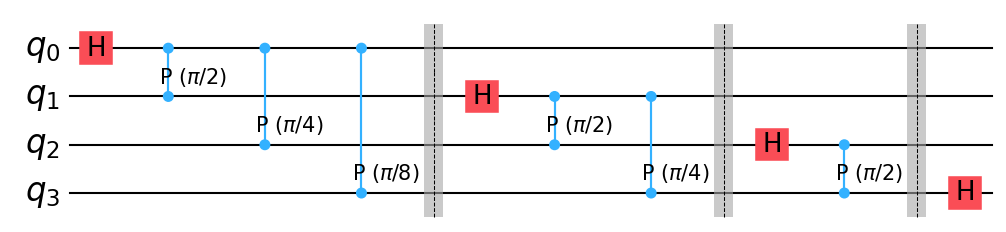
\includegraphics[height=2.5cm]{qft-qiskit.png}
\end{frame}

\begin{frame}
\frametitle{Matrix form of the QFT}

$$\mathrm{QFT}_n = \frac{1}{\sqrt{N}} \begin{bmatrix}
1 & 1 & 1 & 1 & \ldots & 1 \\
1 & \omega & \omega^2 & \omega^3 & \ldots & \omega^{N-1} \\
1 & \omega^2 & \omega^4 & \omega^6 & \ldots & \omega^{2(N-1)} \\
1 & \omega^3 & \omega^6 & \omega^9 & \ldots & \omega^{3(N-1)} \\
\vdots & \vdots & \vdots & \vdots & \ddots & \vdots \\
1 & \omega^{N-1} & \omega^{2(N-1)} & \omega^{3(N-1)} & \ldots & \omega^{(N-1)^2}
\end{bmatrix}$$

where $\omega = e^{2\pi i / N}$ and $N = 2^n$.
\end{frame}



\begin{frame}
    \frametitle{Quantum Phase Estimation}

    The quantum phase estimation algorithm estimates 
    the phase of an eigenvector of a unitary operator.

    \vspace {0.5cm}

    Given a unitary operator $U$ and an eigenvector $\ket{\psi}$ such that 
    $U\ket{\psi} = e^{2\pi i \theta} \ket{\psi}$, 
    the quantum phase estimation algorithm estimates $\theta$.

    \vspace{0.5cm}

    If $\ket{\psi}$ is not an eigenvector of $U$, then the algorithm will
    estimate the phase of a random eigenvector of $U$.
\end{frame}

\begin{frame}
    \frametitle{QPE Circuit - Step 1}
    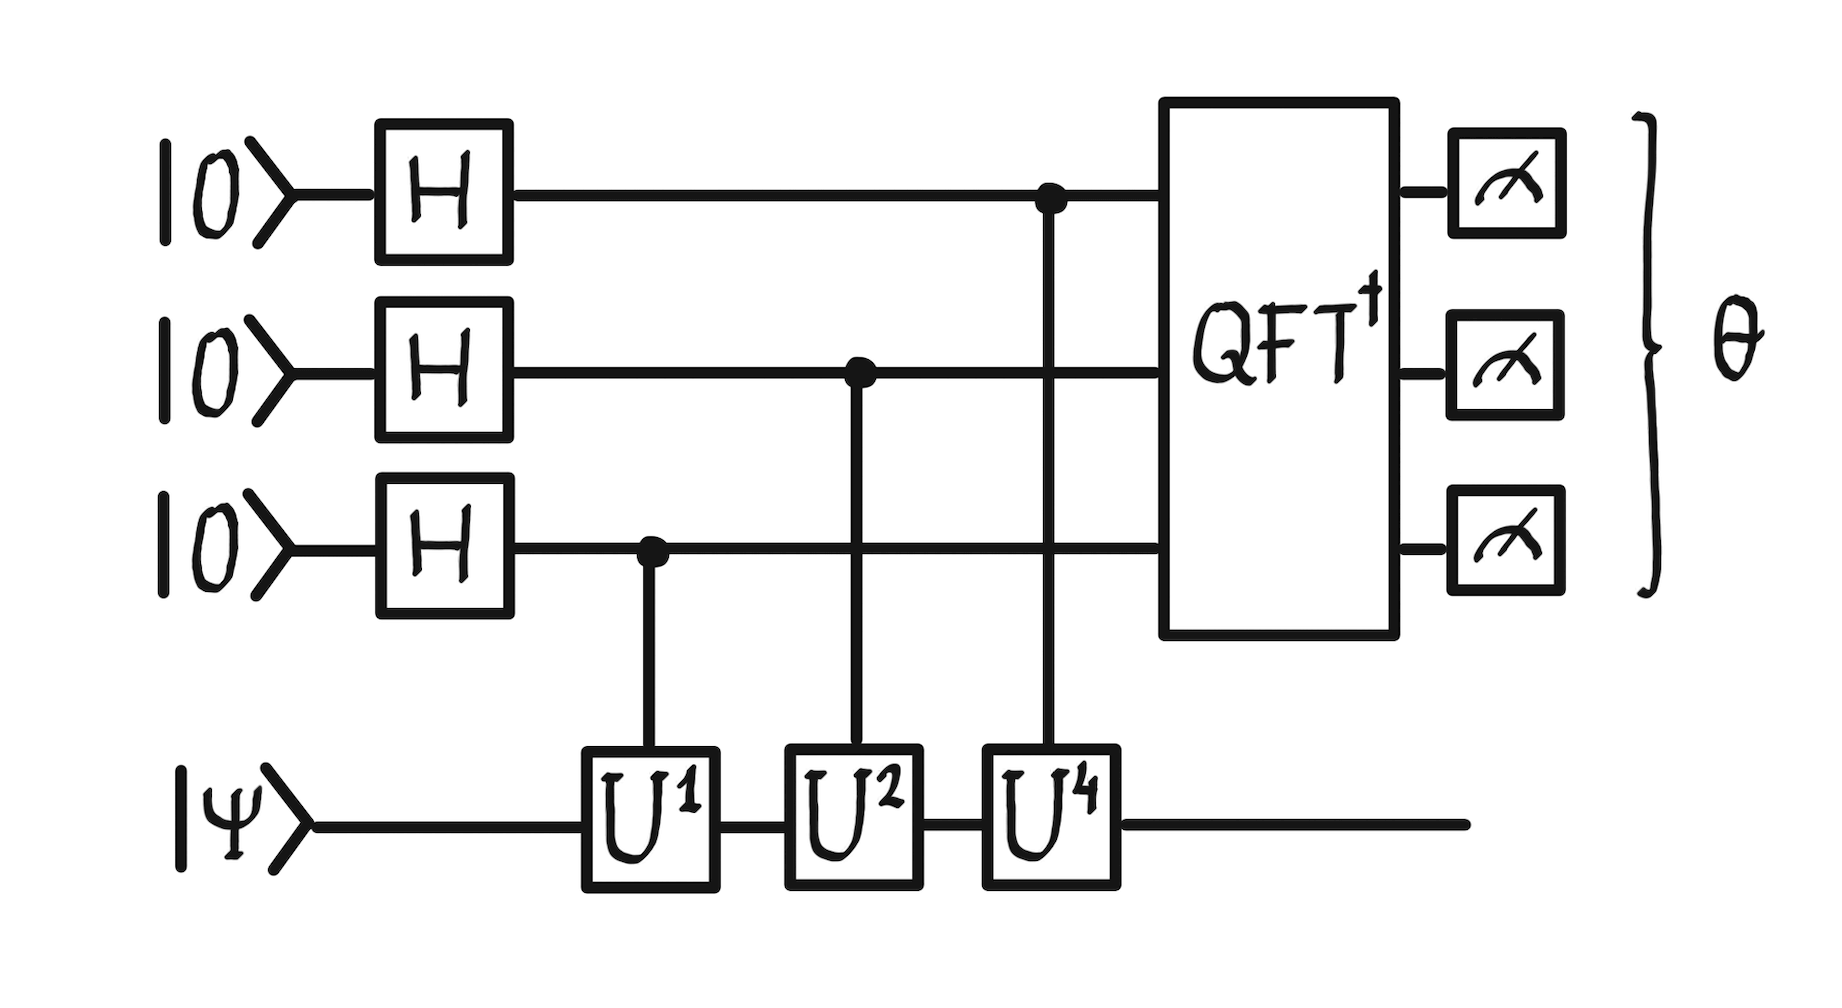
\includegraphics[height=4cm]{qpe.png}

    Step 1: Apply Hadamard gates to the top register,
    placing it in an equal superposition of all basis states.

    $$\ket{0} \mapsto \frac{1}{\sqrt{N}} \sum_{k=0}^{N-1} \ket{k}$$

\end{frame}



\begin{frame}
    \frametitle{QPE Circuit - Step 2}
    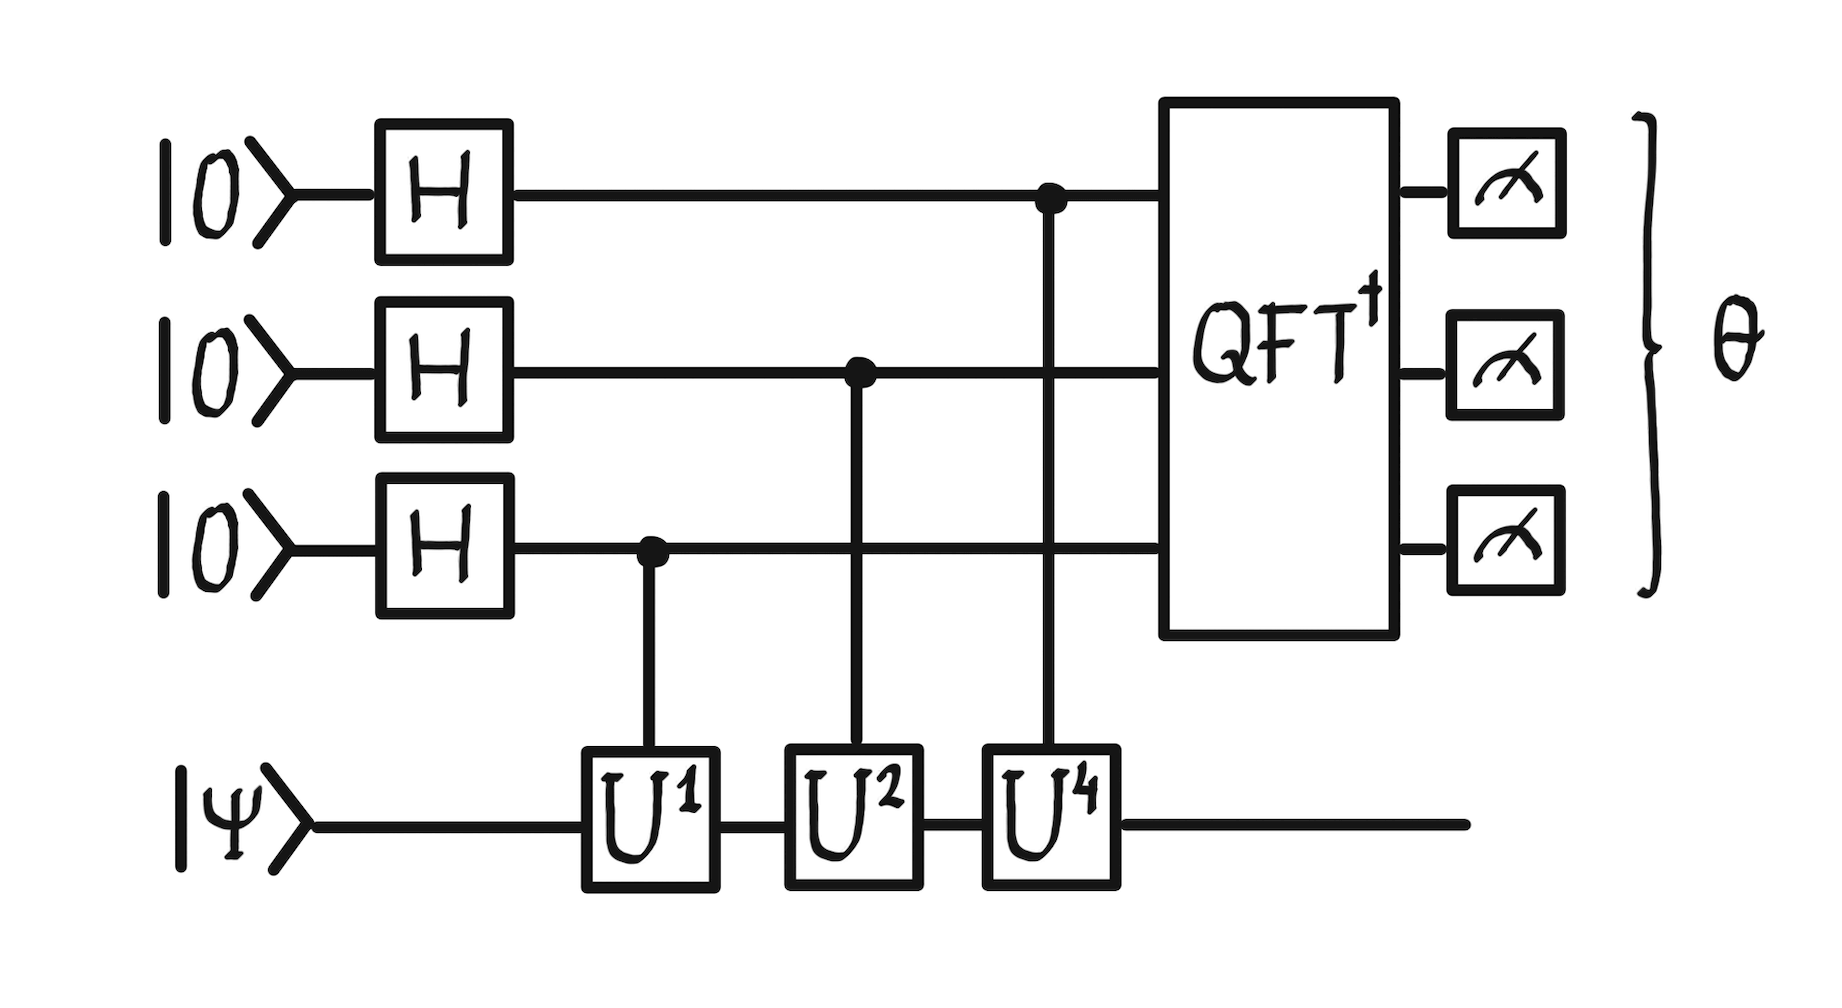
\includegraphics[height=4cm]{qpe.png}

    Step 2: Apply controlled-$U^{2^j}$ gates to the bottom register, 
    controlled on the top register.
  
    % Since the control qubits are in superposition, the phase
    % ``kicks back'' into the top register.
    $$\frac{1}{\sqrt{N}} \sum_{k=0}^{N-1} \ket{k} \ket{\psi} \mapsto
    \frac{1}{\sqrt{N}} \sum_{k=0}^{N-1} \ket{k} U^{k} \ket{\psi}
    = \frac{1}{\sqrt{N}} \sum_{k=0}^{N-1} e^{2\pi i k \theta} \ket{k} \ket{\psi}
    $$
\end{frame}

\begin{frame}
    \frametitle{QPE Circuit - Step 2}
    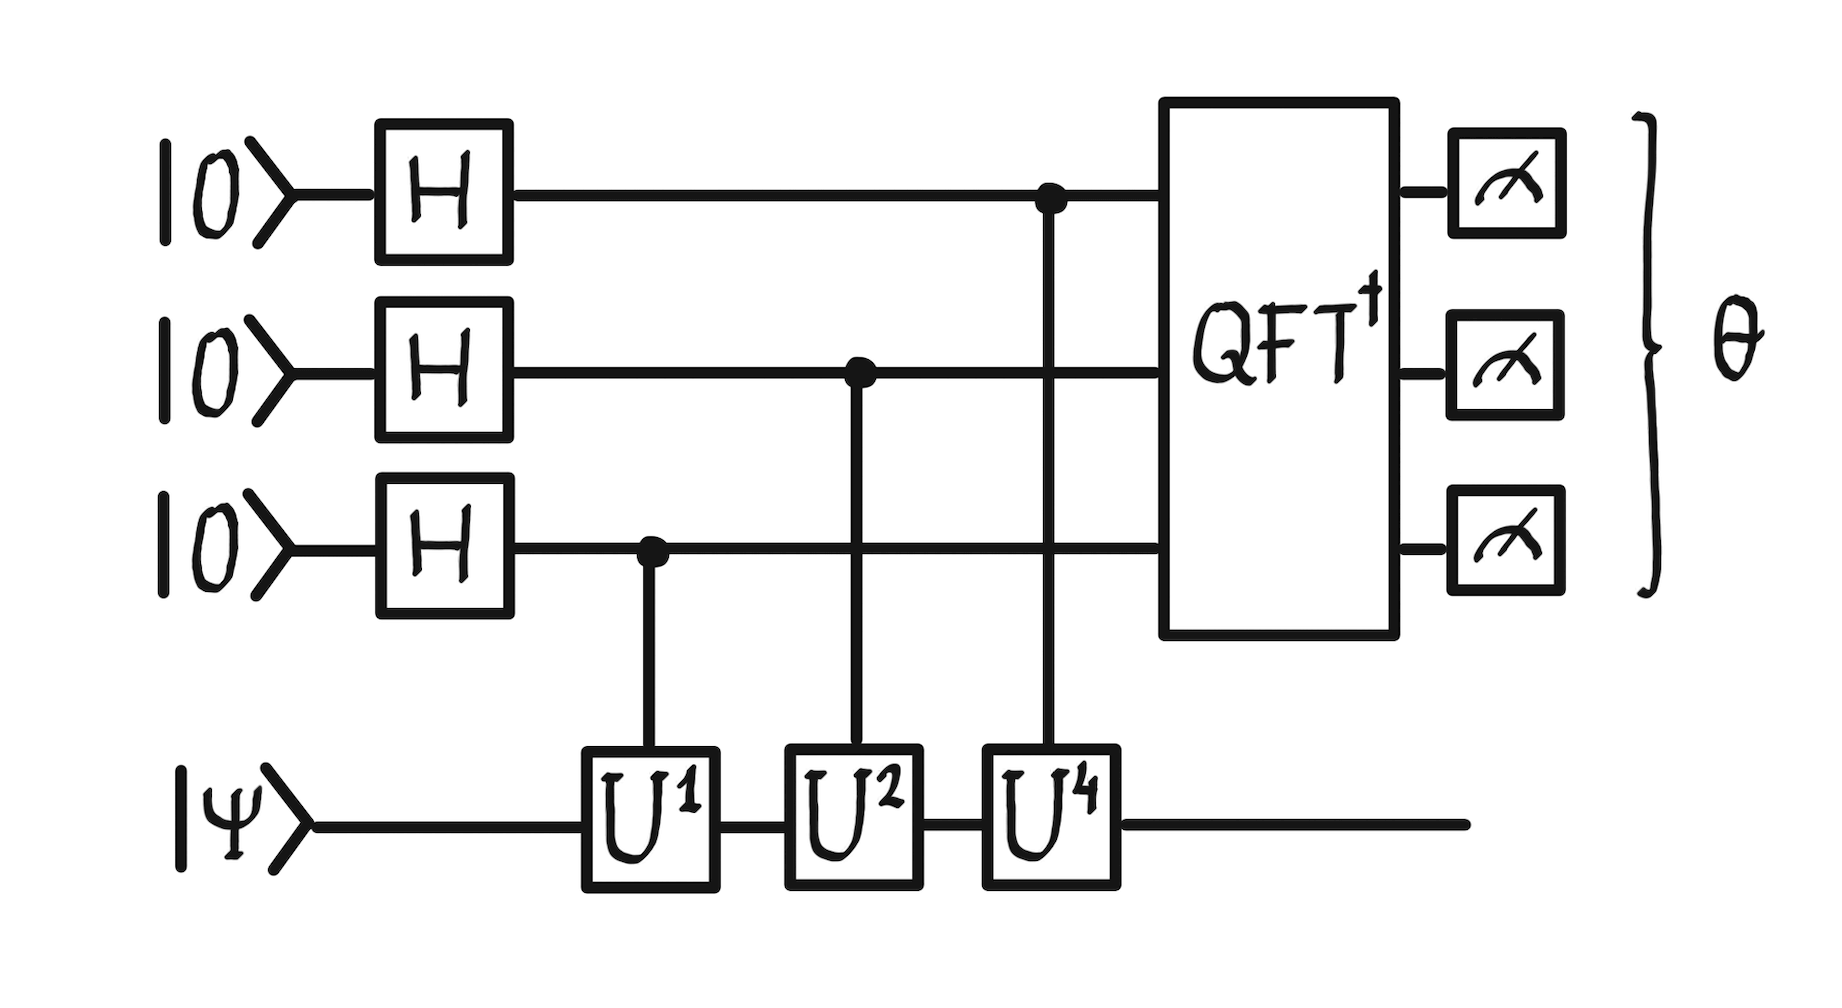
\includegraphics[height=4cm]{qpe.png}

    After applying the controlled-$U^{2^j}$ gates, the system state is
    $$\frac1{\sqrt{N}} \sum_{k=0}^{N-1} \ket{k} \mapsto 
    \frac1{\sqrt{N}} \sum_{k=0}^{N-1} e^{2\pi ik\theta} \ket{k}$$
\end{frame}

\begin{frame}
    \frametitle{QPE Circuit - Step 3}

    Suppose that $\theta = j / N$ for some integer $j$.
    Then the state of the top register after step 2 is
    $$\frac1{\sqrt{N}} \sum_{k=0}^{N-1} e^{2\pi ijk/N} \ket{k}$$

    But this is the same as applying the QFT to the state $\ket{j}$.
    Therefore, applying the inverse QFT to the top register will yield 
    the state $\ket{j}$.
 
    \vspace{0.25cm}
 
    If $N\theta$ is not an integer then $j/N$
    will be an approximation to $\theta$, with high probability.
\end{frame}

\section*{Quantum Order Finding}

\begin{frame}
    \frametitle{Quantum Order Finding}

    Let $M$ be a number to be factored, and let $a$ be a number 
    such that $1 < a < M - 1$ and $\gcd(a, M) = 1$.

    \vspace{0.5cm}

    We wish to find the order $r$ of $a$ mod $M$.
    We can do this using the quantum phase estimation algorithm.

   \vspace{0.5cm}

   Let $U$ be a unitary operator defined by $U\ket{x} = \ket{ax \bmod M}$ 
   for $x < M$, and $U\ket{x} = \ket{x}$ for $x \geq M$.

   \vspace{0.5cm}

   Note that since $U^r = I$, the eigenvalues of $U$ are $e^{2\pi i j / r}$ 
   for $j = 0, 1, \ldots, r-1$.
 
\end{frame}



\begin{frame}
    \frametitle{Quantum Order Finding}

   Apply the QPE algorithm to $U$ and the state $\ket{1}$.

   This yields the state $\ket{c}$, where $c/N \approx j/r$
    for some integer $j$.

    \vspace{0.5cm}

    To compute $r$, we need to find the best approximation to $c/N$
    whose denominator $r$ is less than $M$. This is done using continued fractions.


\end{frame}

\begin{frame}
    \frametitle{Continued fraction example}

    Suppose that we are factoring $M = 21$ with $a=2$ and $N = 2^10 = 1024$.
    QPE yields the approximation $c/N = 171/1024 = 0.1669921875$.
    
    Compute the continued fraction expansion of $171/1024$.
    $$\frac{171}{1024} = [0; 5, 1, 84, 2] = 0 + \cfrac{1}{5 + 
    \cfrac{1}{1 + \cfrac{1}{84 + \cfrac{1}{2}}}}$$
\end{frame}



\begin{frame}
    \frametitle{Continued fraction example}
    Truncating the continued fraction expansion yields the approximation

    $$\frac{j}{r} = [0; 5, 1] = 0 + \cfrac{1}{5 + \cfrac{1}{1}} = \frac{1}{6}$$

    Therefore, the order of 2 mod 21 is 6.

\end{frame}



\end{document}
